\section{Introduction}

\subsection{Problem Definition}
The leisure travelling market is an impactful industry
whose economic importance significantly improves each
year, contributing to 10.4\% of the global GDP in 2019
~\cite{wttc2018travel}. Despite this, planning for a trip to a
foreign city requires a substantial amount of
time-consuming research. As a result, people often
rely on multiple data sources such as travel
brochures, blogs and vlogs to form a holiday plan and
retrieve top-rated points of interest (POI). However,
besides having to compile a timetable independently,
these mediums do not hold the resources to provide
POIs tailored according to the traveller's preferences
and constraints~\cite{DeChoudhury2010}. 

In literature, offering tourists a personalised route
composed of POIs has been defined as the tourist trip
design problem (TTDP). The TTDP is made up of ranking
and selecting POIs that might interest the user and
create a feasible route. Figure~\ref{TTDP} shows an example
of the TTDP,  where a tourist has to form a timetable
that balances between the POI's rating and location
while satisfying the various trip constraints. Section
X provides a detailed review of this problem and its
variants.  

The TTDP is an NP-hard problem where rigorous
algorithms only manage to optimise with a small number
of POIs. Therefore, many approximate algorithms,
namely heuristics and meta-heuristic approaches, work
to converge solutions with complex alternatives to
this problem.

Nevertheless, the few existing systems that provide
users with an itinerary or route require a lengthy
process of manually gathering the users' likes and
constraints or information from past trips. 
Can a system automate the process of formulating what
POI categories a tourist likes?

\begin{figure}[h]
\centering
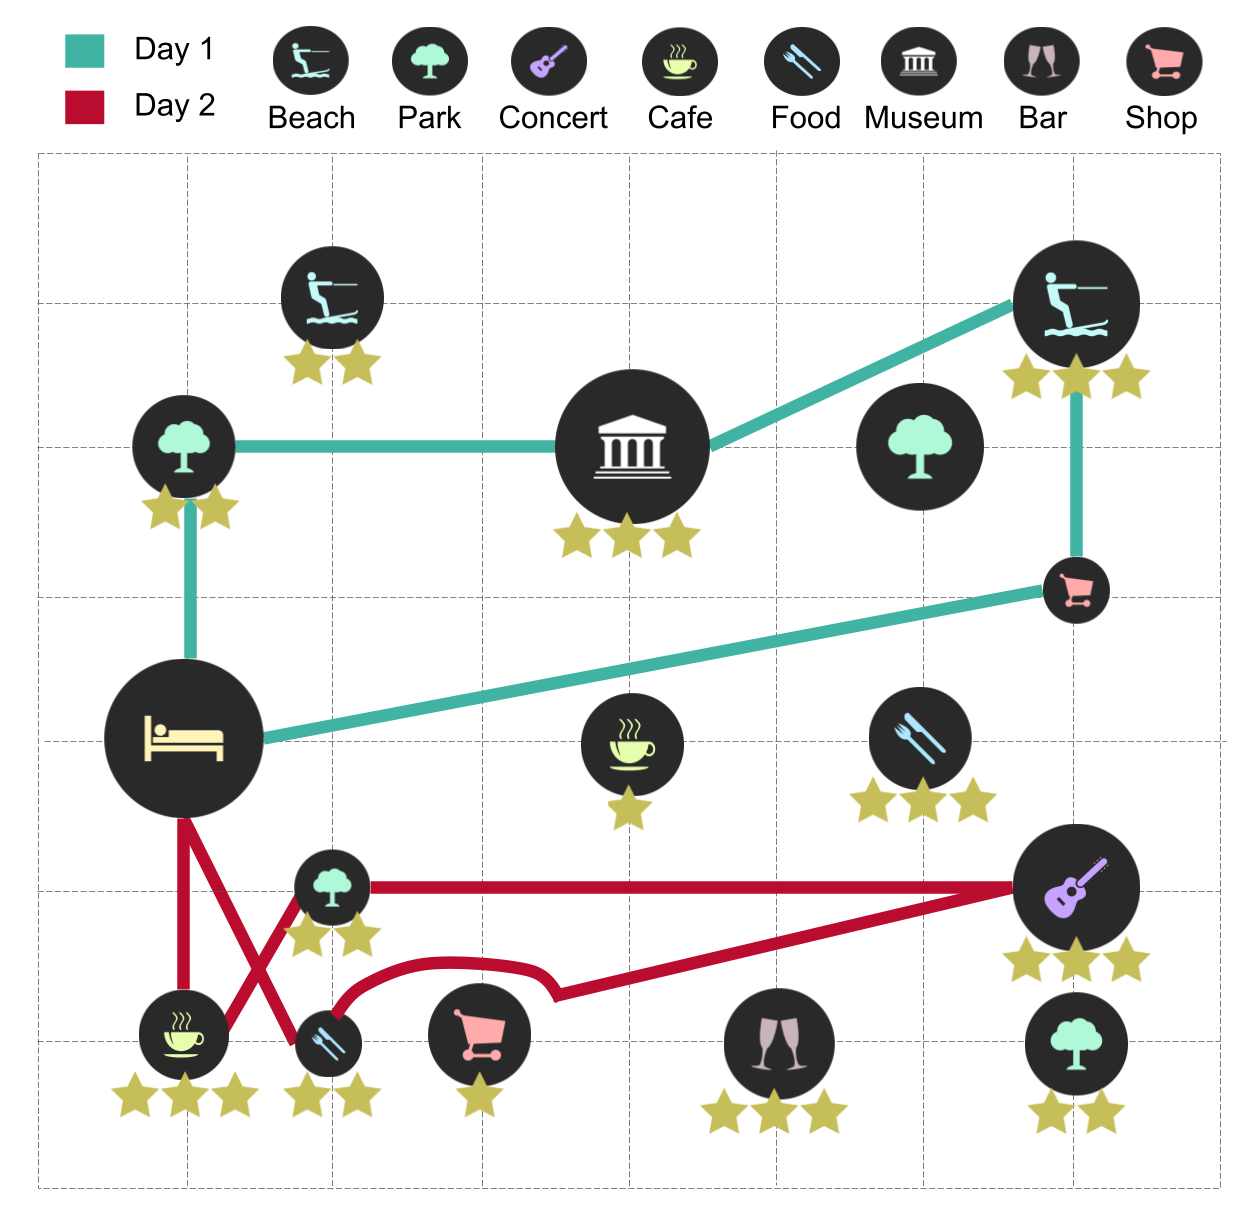
\includegraphics[width=0.75\textwidth]{TTDP.png}
\caption{Example of a tourists planning problem}
\label{TTDP}
\end{figure}

\subsection{Proposed Solution}

To address this problem, we present an application
that helps tourists travel by providing them with a
complete itinerary for their upcoming holiday using
several optimisation algorithms. 

With the prevalence of social media and data-driven
approaches, we also automate gathering users' POI
desires by scanning their social media profile using
machine learning classification approaches.

The results from the evaluation (insert section ref)
show that we were able to use convolutional neural
networks (CNN) to classify the user's photos into a
travel interest vector for automatically gathering the
preferences. We were also able to provide optimisation
techniques that converge to the timetables with the
best scores given a set of tourist constraints.
In-depth semi-structured interviews with several
participants continued to provide us with further
detail on the accuracy of the user profiling algorithm
and the resulting timetables. 

\subsection{Motivation}

Our primary motivation behind this work is
to introduce the automatic retrieval of user
preferences for a travel planner application. This app
will heavily benefit the tourists by providing them
with something quick and easy to use. We believe that
this approach is better than bombarding the tourist
with many questions to understand the users' likings.
We were also motivated by the idea of providing one
centralised system which organises the whole holiday
rather than having to spend time searching through the
excessive amount of data online. 

\subsection{Why the problem is non-trivial}

Existing algorithms and tourist planners use
heuristics to optimise solutions for the timetable
problem and are achievable in polynomial time (cite
here). 

Automatic user preference gathering is a beneficial
technique used by businesses to advertise their
products by targeting only a specific audience (cite
here).  

The problem is non-trivial since we combine both
technologies to provide one system.

\subsection{Aims and Objectives}

This dissertation aims to build an application that
generates a personalised holiday plan according to the
user's travel dates and constraints.


\begin{itemize}
    \item \textbf{Objective 1 (O1)}: Investigate techniques to build travel interest
    profiles automatically from social media interactions.  
    \item \textbf{Objective 2 (O2)}: Explore different optimisation algorithms for
    building personalised travel itineraries using the
    generated travel interest profiles. 
    \item \textbf{Objective 3 (O3)}: Evaluate the
    performance of the personalised travel itinerary
    generator with real users through in-depth
    semi-structured interviews. 

\end{itemize}

We will conduct the interviews by generating a
timetable for a holiday in Malta so that the
interviewees would have prior knowledge of the POIs.

\subsection{Document Structure}

This dissertation is structured as follows; Section 2
discusses related work relating to existing TTDP
solutions and automatic user preference gathering.
Section 3 demonstrates the steps taken to create the
whole application along with its underlying mechanism.
Section 4 will evaluate the performance of the
convolutional neural networks, the optimisation
algorithms and discuss the interview's outcomes.
Finally, section 5 will address the findings obtained
from this research concerning the objectives and some
future improvements.

